\documentclass[10pt,oneside]{article}

\usepackage[utf8]{inputenc}
\usepackage[T1]{fontenc}
\usepackage[default]{raleway}
\usepackage[a4paper,left=1.45cm,right=1.45cm,top=1.25cm,bottom=1.25cm]{geometry}
\usepackage{array}
\usepackage{fancyhdr}
\usepackage{graphicx}
\usepackage[hidelinks]{hyperref}
\usepackage{longtable}
\usepackage{microtype}
\usepackage{tcolorbox}
\usepackage{xcolor}

\graphicspath{{./Figs/}}

\definecolor{AcademicNavy}{HTML}{172638}
\definecolor{AcademicBlue}{HTML}{365F91}
\definecolor{AcademicGold}{HTML}{B48B45}
\definecolor{AcademicMuted}{HTML}{607083}
\definecolor{AcademicPaper}{HTML}{F5F2EB}

\hypersetup{
  colorlinks=true,
  urlcolor=AcademicBlue,
  linkcolor=AcademicBlue
}

\setlength{\parindent}{0pt}
\setlength{\parskip}{0pt}
\renewcommand{\arraystretch}{1.08}
\renewcommand{\headrulewidth}{0pt}

\pagestyle{fancy}
\fancyhf{}
\fancyfoot[L]{\small\color{AcademicMuted}Chunhui Wei}
\fancyfoot[R]{\small\color{AcademicMuted}\thepage}

\newcommand{\sectionheading}[1]{%
  \vspace{0.35cm}
  {\Large\bfseries\color{AcademicNavy}#1}\par
  \vspace{0.08cm}
  {\color{AcademicGold}\rule{\textwidth}{1.1pt}}
  \vspace{0.12cm}
}

\newcommand{\cventry}[5]{%
  \textcolor{AcademicBlue}{\textbf{#1}} &
  \textbf{\color{AcademicNavy}#2}\hfill{\small\textit{#4}}\newline
  \textit{#3}\newline
  #5\\[0.28cm]
}

\newcommand{\publication}[5]{%
  \textcolor{AcademicBlue}{\textbf{#1}} &
  \textbf{\color{AcademicNavy}#2}\newline
  #3\newline
  \textit{#4}\hfill #5\\[0.3cm]
}

\begin{document}
\thispagestyle{fancy}

\begin{tcolorbox}[
  boxrule=0pt,
  arc=0pt,
  colback=AcademicPaper,
  left=0.55cm,
  right=0.45cm,
  top=0.45cm,
  bottom=0.45cm
]
  \begin{minipage}[t]{0.68\linewidth}
  \vspace{0pt}
  {\fontsize{27}{30}\selectfont\bfseries\color{AcademicNavy}Chunhui Wei}\par
  \vspace{0.08cm}
  {\large\color{AcademicBlue}Ph.D. Student in Mathematics}\par
  \vspace{0.28cm}
  Zhejiang University, Hangzhou, China\par
  Ph.D. Supervisor: Professor Song Sun\par
  \vspace{0.25cm}
  \href{mailto:chunhuiwei@zju.edu.cn}{chunhuiwei@zju.edu.cn}\par
  \href{https://chunhuiwei736.github.io}{chunhuiwei736.github.io}
  \end{minipage}
  \hfill
  \begin{minipage}[t]{0.24\linewidth}
  \vspace{0pt}
  \centering
  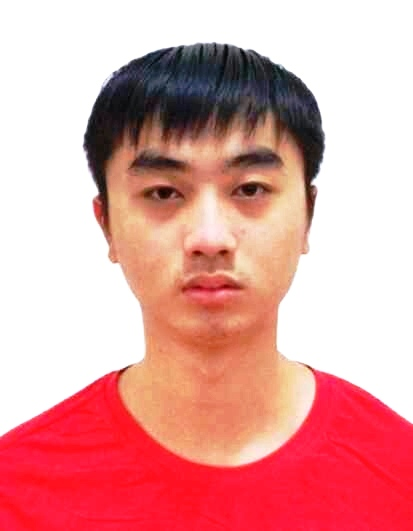
\includegraphics[width=2.85cm]{picture.jpg}
  \end{minipage}
\end{tcolorbox}

\vspace{0.22cm}
{\color{AcademicMuted}
I work in geometry and topology, with interests in complex geometry, complex algebraic
geometry, and algebraic K-theory.
}

\sectionheading{Education}
\begin{longtable}{@{}p{0.17\textwidth} p{0.79\textwidth}@{}}
  \cventry{2026--Present}
    {Ph.D. in Mathematics}
    {Zhejiang University}
    {Hangzhou, China}
    {\textbf{Supervisor:} Professor Song Sun}

  \cventry{2024--2025}
    {Master of Science, Mathematics and Statistics}
    {University of Melbourne}
    {Melbourne, Australia}
    {\textbf{Thesis:} \textit{Remarks on Semi-topological Quillen-Lichtenbaum Conjecture}\newline
     \textbf{Supervisor:} Professor Christian Haesemeyer}

  \cventry{2019--2023}
    {Bachelor of Science, Mathematics and Applied Mathematics}
    {University of Science and Technology of China, School of Gifted Young}
    {Hefei, China}
    {\textbf{Thesis:} \textit{Reduced solutions of the SU-Toda system}\newline
     \textbf{Advisor:} Associate Professor Bin Xu}
\end{longtable}

\sectionheading{Publications and Preprints}
\begin{longtable}{@{}p{0.11\textwidth} p{0.85\textwidth}@{}}
  \publication{2026}
    {Noncommutative Quillen-Lichtenbaum Conjecture}
    {\textbf{Chunhui Wei}}
    {Preprint}
    {\href{https://arxiv.org/abs/2604.27373}{arXiv:2604.27373}}

  \publication{2026}
    {D\'evissage for Algebraic K-theory of Small Stable $\infty$-categories}
    {\textbf{Chunhui Wei}}
    {Preprint}
    {\href{https://arxiv.org/abs/2601.14626}{arXiv:2601.14626}}

  \publication{2026}
    {Solutions to SU$(n+1)$ Toda system generated by spherical metrics}
    {Yiqian Shi, \textbf{Chunhui Wei}, and Bin Xu}
    {Journal of Functional Analysis, 290(1), 111197}
    {\href{https://doi.org/10.1016/j.jfa.2025.111197}{DOI}}
\end{longtable}

\sectionheading{Research Experience}
\begin{longtable}{@{}p{0.17\textwidth} p{0.79\textwidth}@{}}
  \cventry{2026}
    {Visiting Scholar}
    {Institute for Advanced Study in Mathematics, Zhejiang University}
    {Hangzhou, China}
    {Worked with Professor Song Sun on K\"ahler geometry.}

  \cventry{2024--2025}
    {Research Project}
    {University of Melbourne}
    {Melbourne, Australia}
    {Studied the topological K-theory of complex noncommutative spaces under the
     supervision of Professor Christian Haesemeyer.}
\end{longtable}

\newpage
\sectionheading{Research Experience (continued)}
\begin{longtable}{@{}p{0.17\textwidth} p{0.79\textwidth}@{}}
  \cventry{2023}
    {Research Assistant}
    {CAS Wu Wen-Tsun Key Laboratory of Mathematics, USTC}
    {Hefei, China}
    {Worked with Professor Bin Xu on Toda systems with regular singularities on
     complex manifolds.}

  \cventry{2022--2023}
    {College Student Research Program}
    {University of Science and Technology of China}
    {Hefei, China}
    {Studied reduced solutions of the SU-Toda system under the direction of
     Associate Professor Bin Xu.}

  \cventry{2020--2022}
    {National Innovation and Entrepreneurship Training Program}
    {University of Science and Technology of China}
    {Hefei, China}
    {Studied the SU-Toda system with singularities on the Riemann sphere as a
     team member advised by Associate Professor Bin Xu.}
\end{longtable}

\sectionheading{Technical Skills}
\begin{longtable}{@{}p{0.17\textwidth} p{0.79\textwidth}@{}}
  \textcolor{AcademicBlue}{\textbf{Research}} &
    \LaTeX, Overleaf, Mathematica, MATLAB\\[0.18cm]
  \textcolor{AcademicBlue}{\textbf{Programming}} &
    Python, C, R, HTML\\[0.18cm]
  \textcolor{AcademicBlue}{\textbf{Languages}} &
    Chinese (native), English (advanced)
\end{longtable}

\vfill
{\small\color{AcademicMuted}Last updated: July 2026}

\end{document}
